\documentclass[11pt,letter]{article}
\usepackage[top=1.00in, bottom=1.0in, left=1.1in, right=1.1in]{geometry}
\renewcommand{\baselinestretch}{1.1}
\usepackage[
singlelinecheck=false % <-- important
]{caption}
\usepackage{hyperref}%helps with the email address 
\usepackage{graphicx} %including pictures 

\def\labelitemi{--}
\parindent=0pt

\def\labelitemi{--}
\parindent=0pt

\newenvironment{smitemize}{
\begin{itemize}
  \setlength{\itemsep}{0pt}
  \setlength{\parskip}{0.8pt}
  \setlength{\parsep}{0pt}}
{\end{itemize}
}

\graphicspath{ {./protPhotos/} }% tell latex where to find photos 

\begin{document}
\bibliographystyle{/Users/Lizzie/Documents/EndnoteRelated/Bibtex/styles/besjournals}
\renewcommand{\refname}{\CHead{}}

\title{Wolkovich Phenology Monitoring Protocol\\
Dark Horse Vineyard}
\date{ }
\maketitle
\tableofcontents
\newpage
\section{The short version} % try to keep to one page or under
Here we want a short bulleted list .... that covers:
\emph{Read the whole document before you first go out, or if you have questions. But here we provide short version to review more regularly.}
\begin{smitemize}
\item Try to visit each flagged vine at least once a week.
\item Supplies: datasheets, clipboard, pencil, Plant ID information
\item 24 plants per block, 3 buds/clusters per plant
\item Plants should be labeled with their Plant ID number
\item Buds are numbered 1 to 3. Bud 1 is always the most southern or eastern bud.
\item Budburst and leaf-out: Record Eichorn-Lorenz stages
\item Flowering: Record percent flowering
\item Veraison: Record percent veraison
\item Check -- did you record data on 96 plants (288 buds/clusters)?
\item Back in the office: scan datasheet, label photos. Send to Mira Garner.
\end{smitemize}
\newpage

\section{Objectives}
We aim to characterize the phenology of a large number of winegrape varieties planted in vineyards around the Okanagan Valley in BC. Our primary goal is to improve grower models of phenological timing with relation to climate. To this end, we aim to monitor a diversity of varieties that capture differences in phenology. We will record the timing of phenological events for selected vines for 2-3 growing seasons from budburst through the summer to veraison. We will also take Brix measurements several times after veraison. Due to the limitations on travel and fieldwork during Corvid-19, we are not able to monitor the plants throughout the summer this year. Mike Watson has kindly agreed to some surveying through Arterra employees at the Dark Horse vineyard.

\section{Sampling population at Dark Horse}
\begin{figure}%this will always show at this point 
  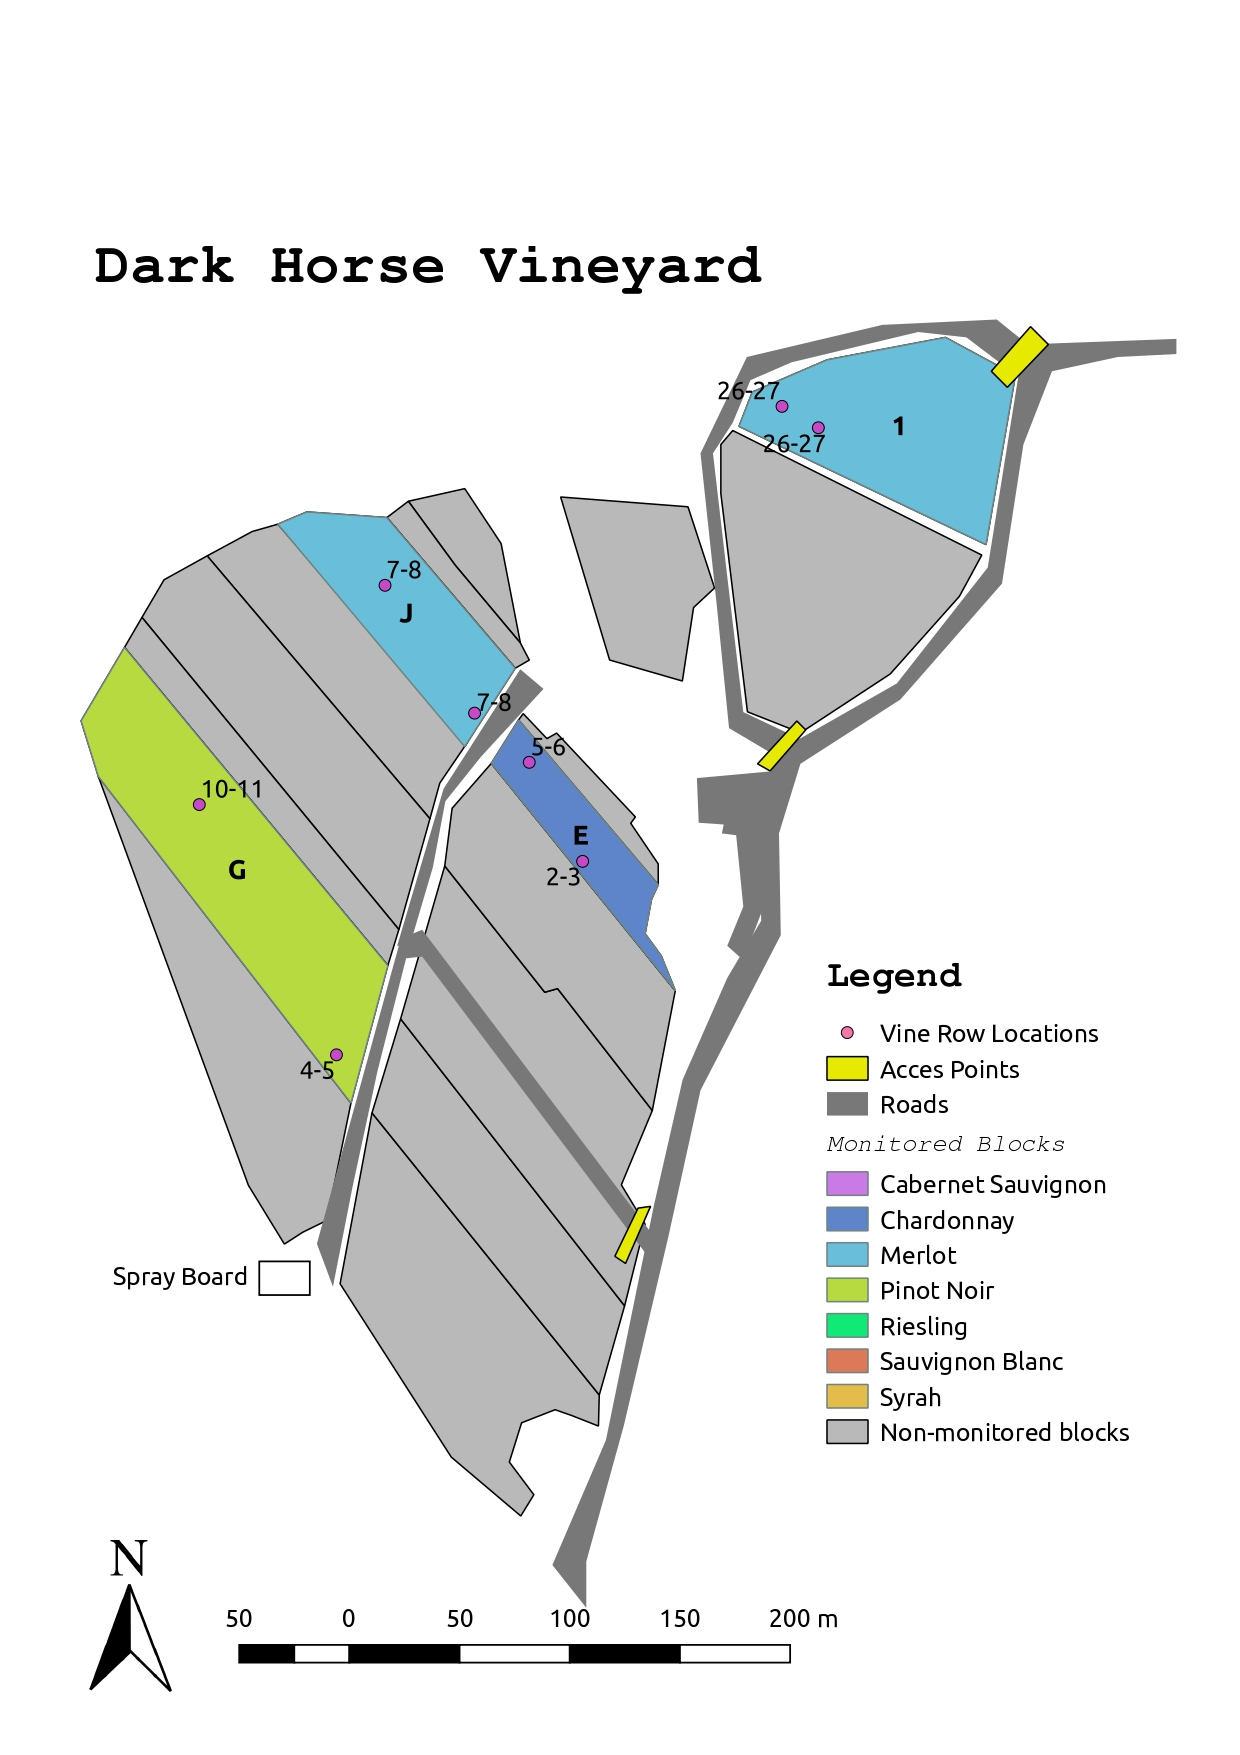
\includegraphics[width=\linewidth]{DH_map.jpg}
  \caption{A may of the location of the vines we are sampling. Each point is a collection of 12 vines labeled with the row numbers of the vines}
  \label{fig:DH_map}
\end{figure}

We are monitoring vines in the following locations: \\
Block G - rows 4-5 south end, 10-11 middle \\
Block J - rows 7-8 south end and middle \\
Block E - rows 5-6 north end, 2-3 middle \\
Block 1 - rows 26-27 west end and middle \\

See Figure \ref{fig:DH_map} for a map of the locations. \\

There are 6 plants on each row at each location so with the adjacent row, there will be groups of 12 flagged plants. More information about location and individual Plant ID numbers is in the spreadsheet called darkhorsePlantID.csv

\section{Overview}
\begin{enumerate}
  \item Lizzie's team (Mira and Faith) flagged vines and started surveying phenology in early May. We were not out early enough for budburst. 
  \item We will aimed to monitor four phenological stages, but missed budburst:
  \begin{enumerate}
	\item Budburst (approximately mid April/early May). Until EL stage 9, record the EL stage of buds on three spurs. Once EL stage is at 9 you can stop recording until flowering starts (note that you may need to record higher than stage 9 at times in order to record whatever stage you see after 8, even if it is 12 or such if you have not yet recorded stage 9, more on this below).
	\item Bloom (approximately May/early June)
  	\item Veraison (approximately mid July-mid August)
  	\item Ripening (Brix - approximately mid August-end September)
  \end{enumerate}
  \item We hope to bring someone back at least for Brix sampling, so we mostly need help with flowering and veraison monitoring. 
  \item We aim to sample at least once a week. If you have more time, especially if it has been a warm week, then twice a week would be even better.

\end{enumerate}


\begin{figure}%this will always show at this point 
  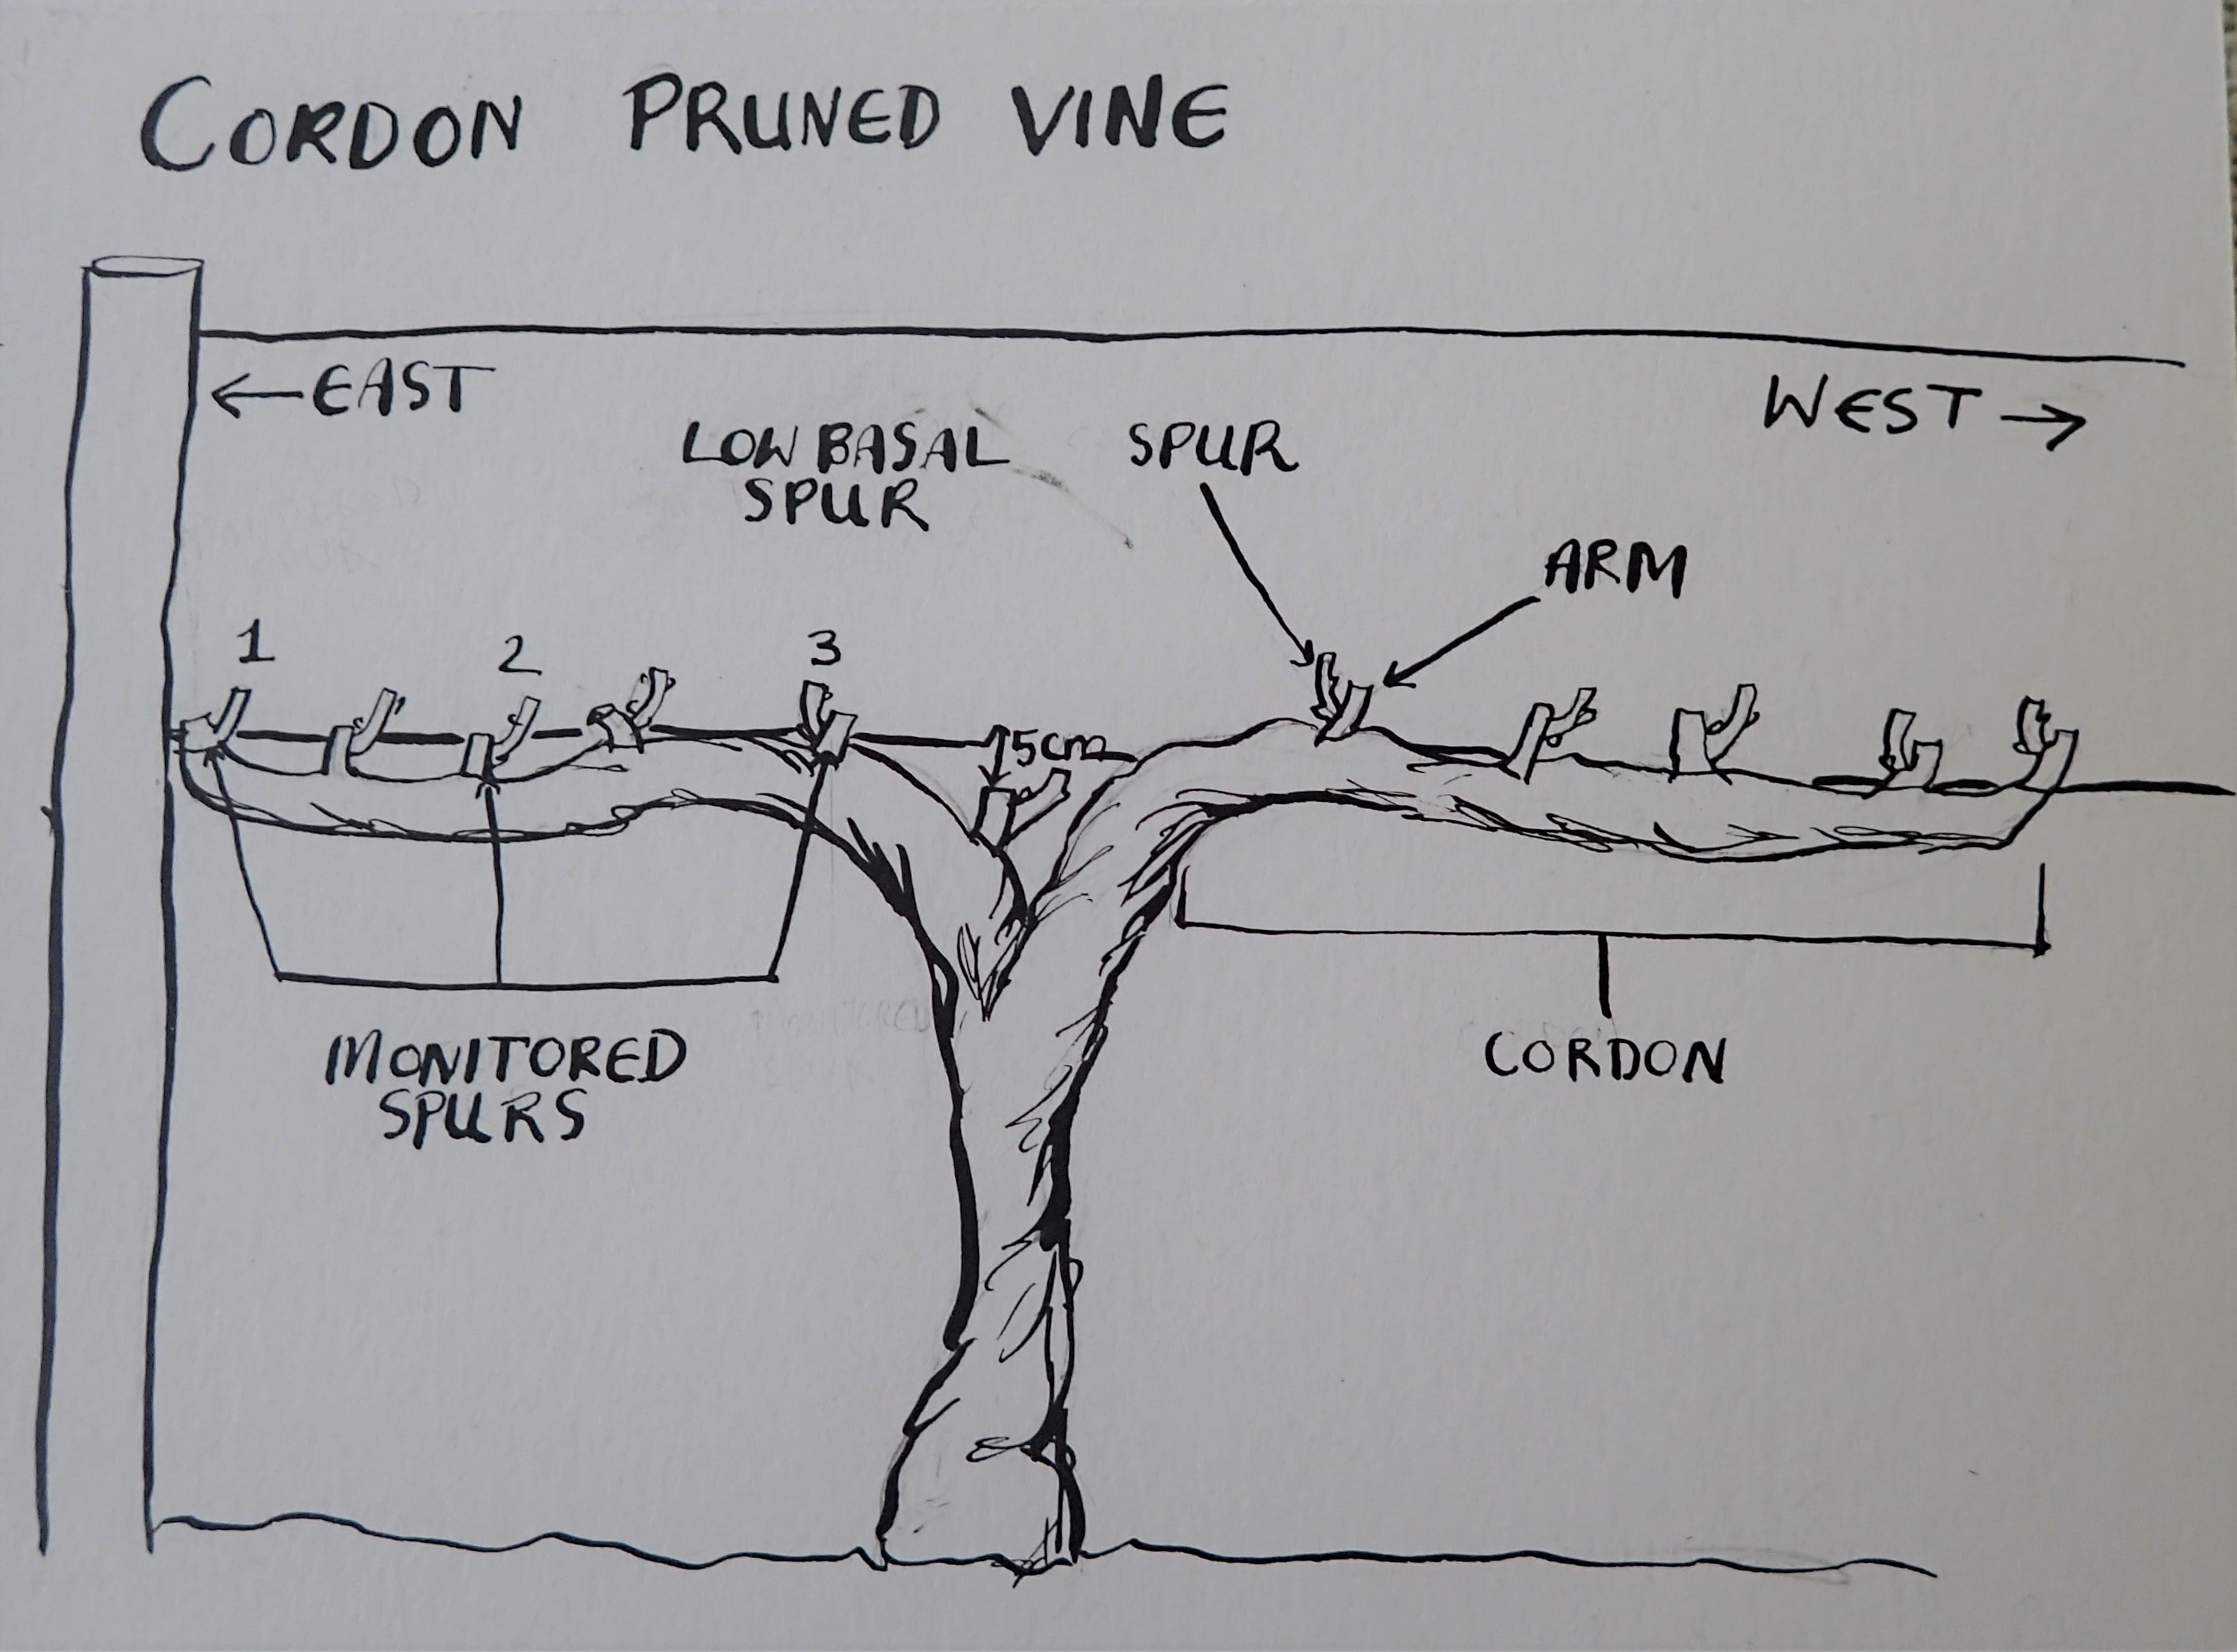
\includegraphics[width=\linewidth]{CordonPruned.jpg}
  \caption{A diagram of a cordon pruned vine, showing which spurs we would monitor. Buds were numbered from east to west or south to north, and any spur that's base was more than 5cm below the wire the cordon was trained on was not sampled.}
  \label{fig:CordonPruned}
\end{figure}

\begin{figure}%this will always show at this point 
  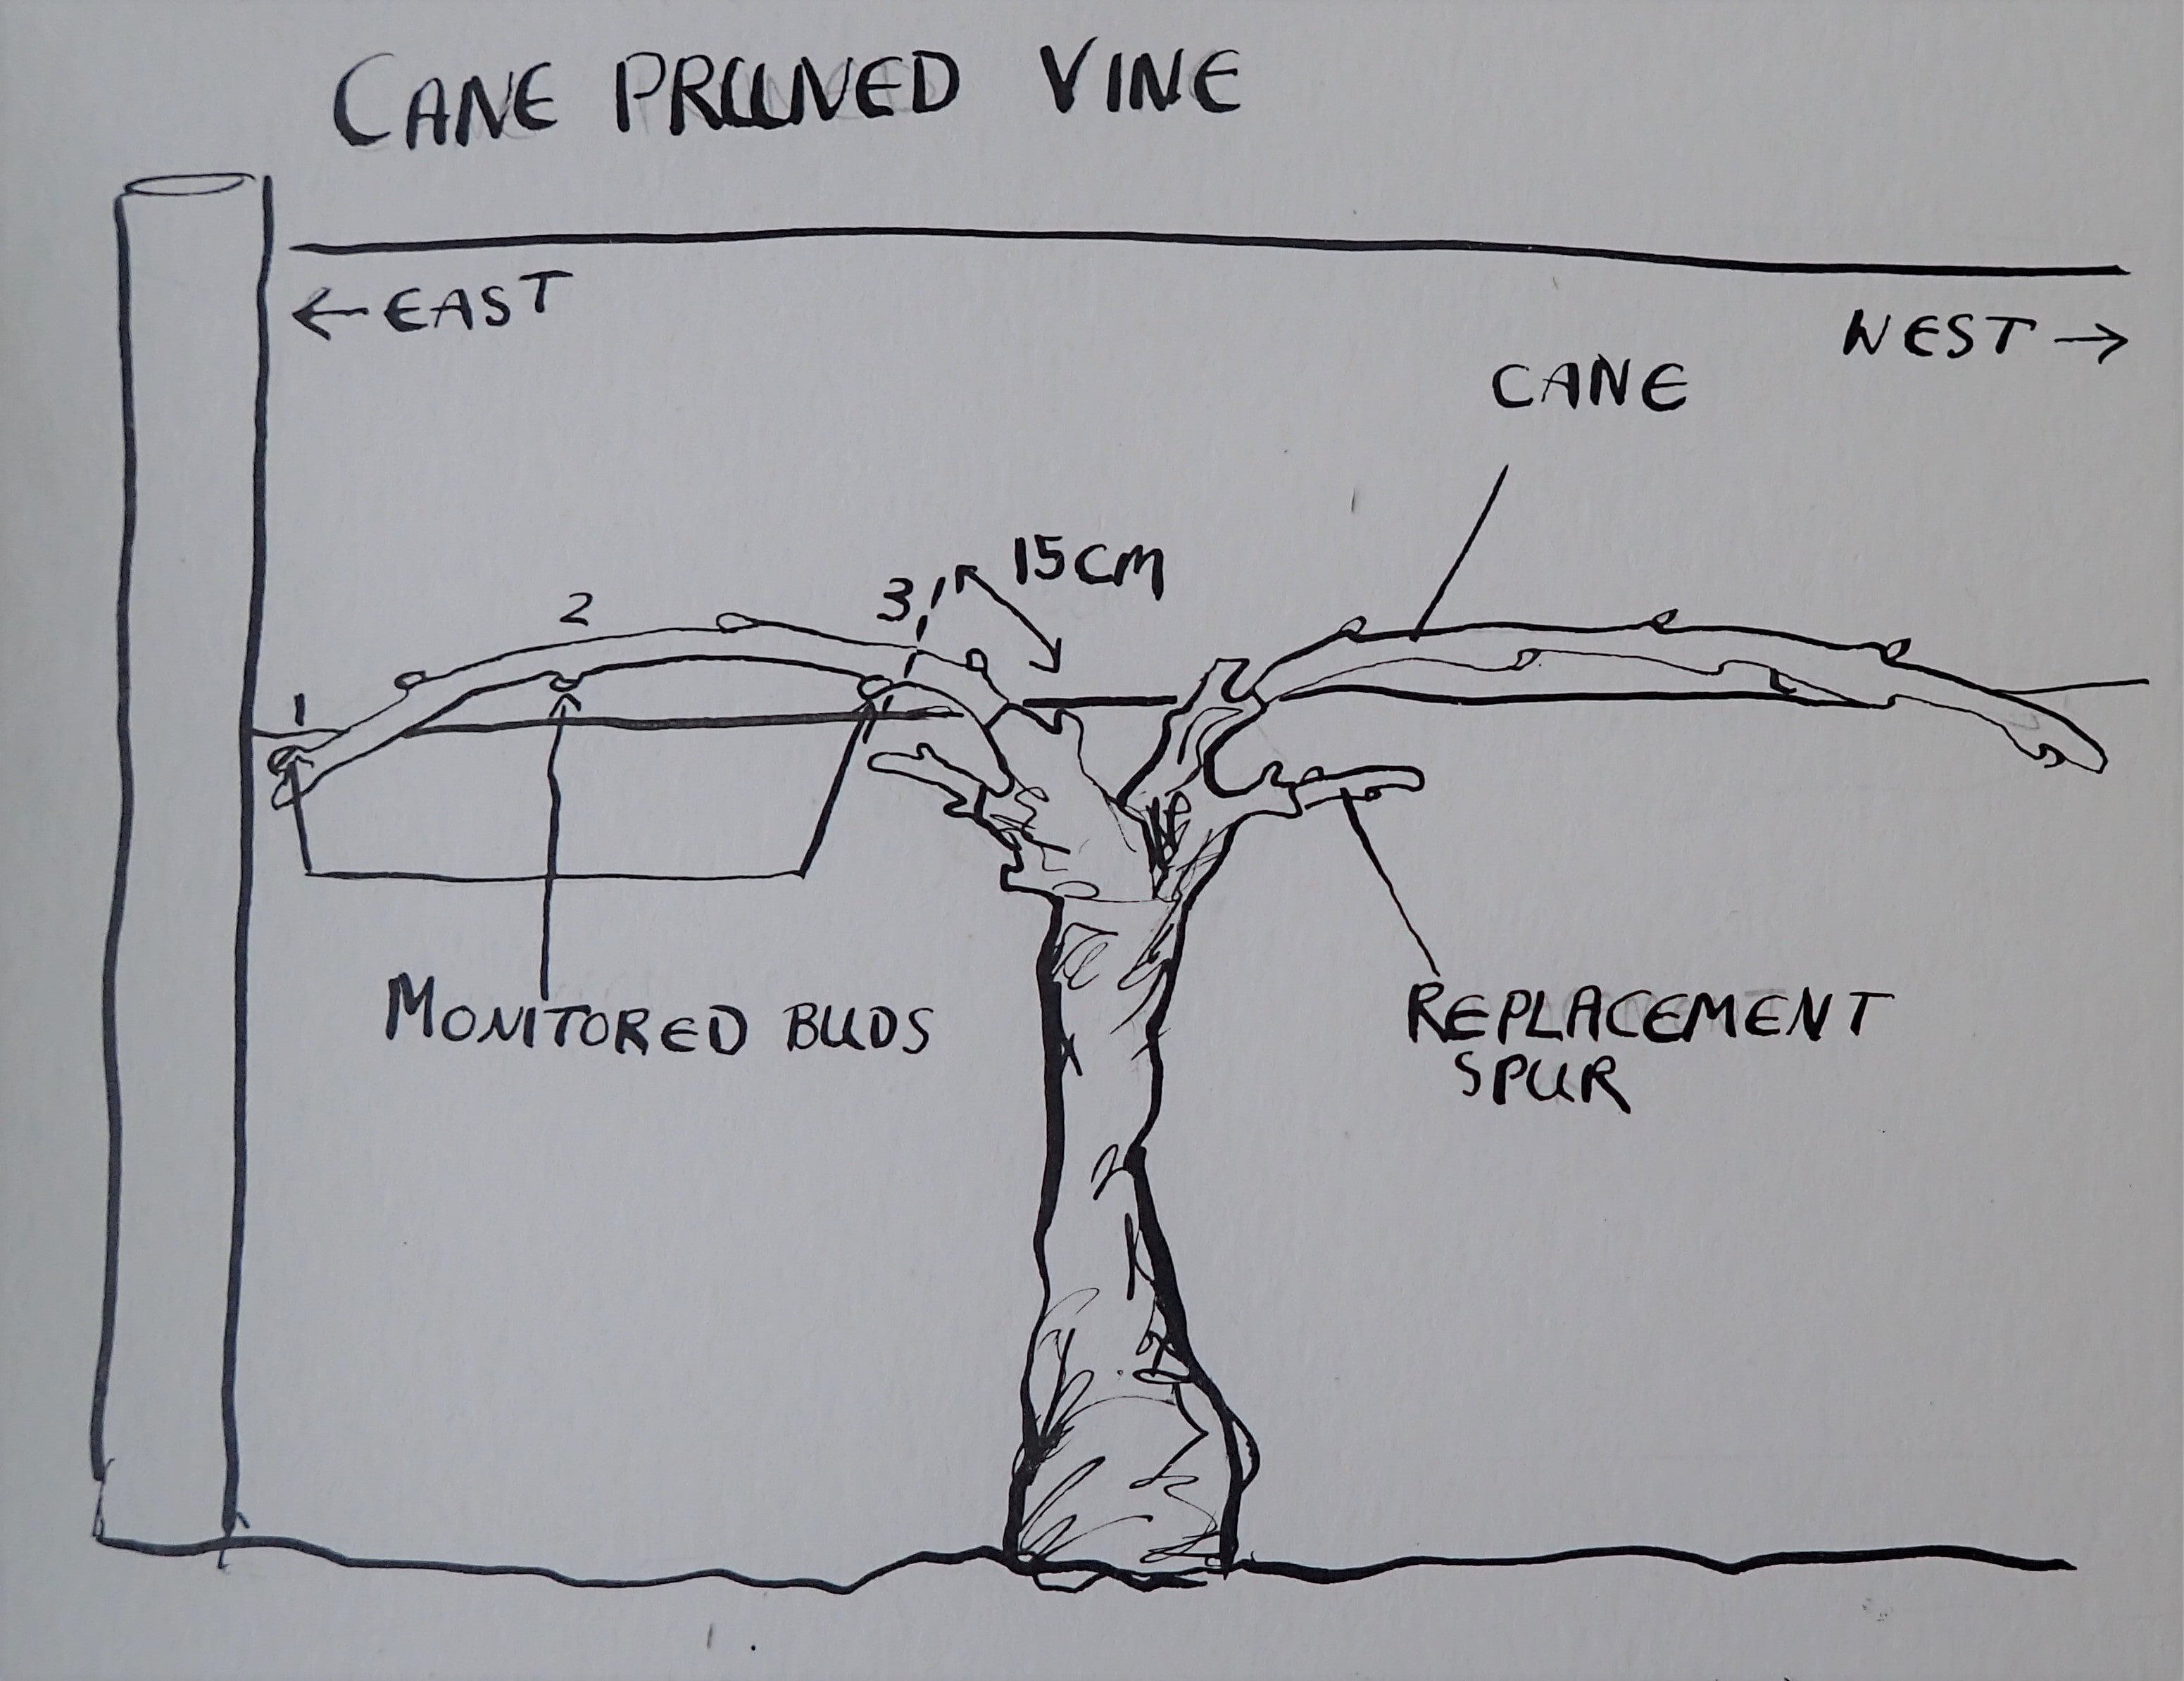
\includegraphics[width=\linewidth]{CanePruned.jpg}
  \caption{A diagram of a cane pruned vine, with the buds we would monitor and their numbering shown. Note that we do not sample buds too close to the head of the vine.}
  \label{fig:CanePruned}
\end{figure}

\begin{figure}%this will always show at this point 
  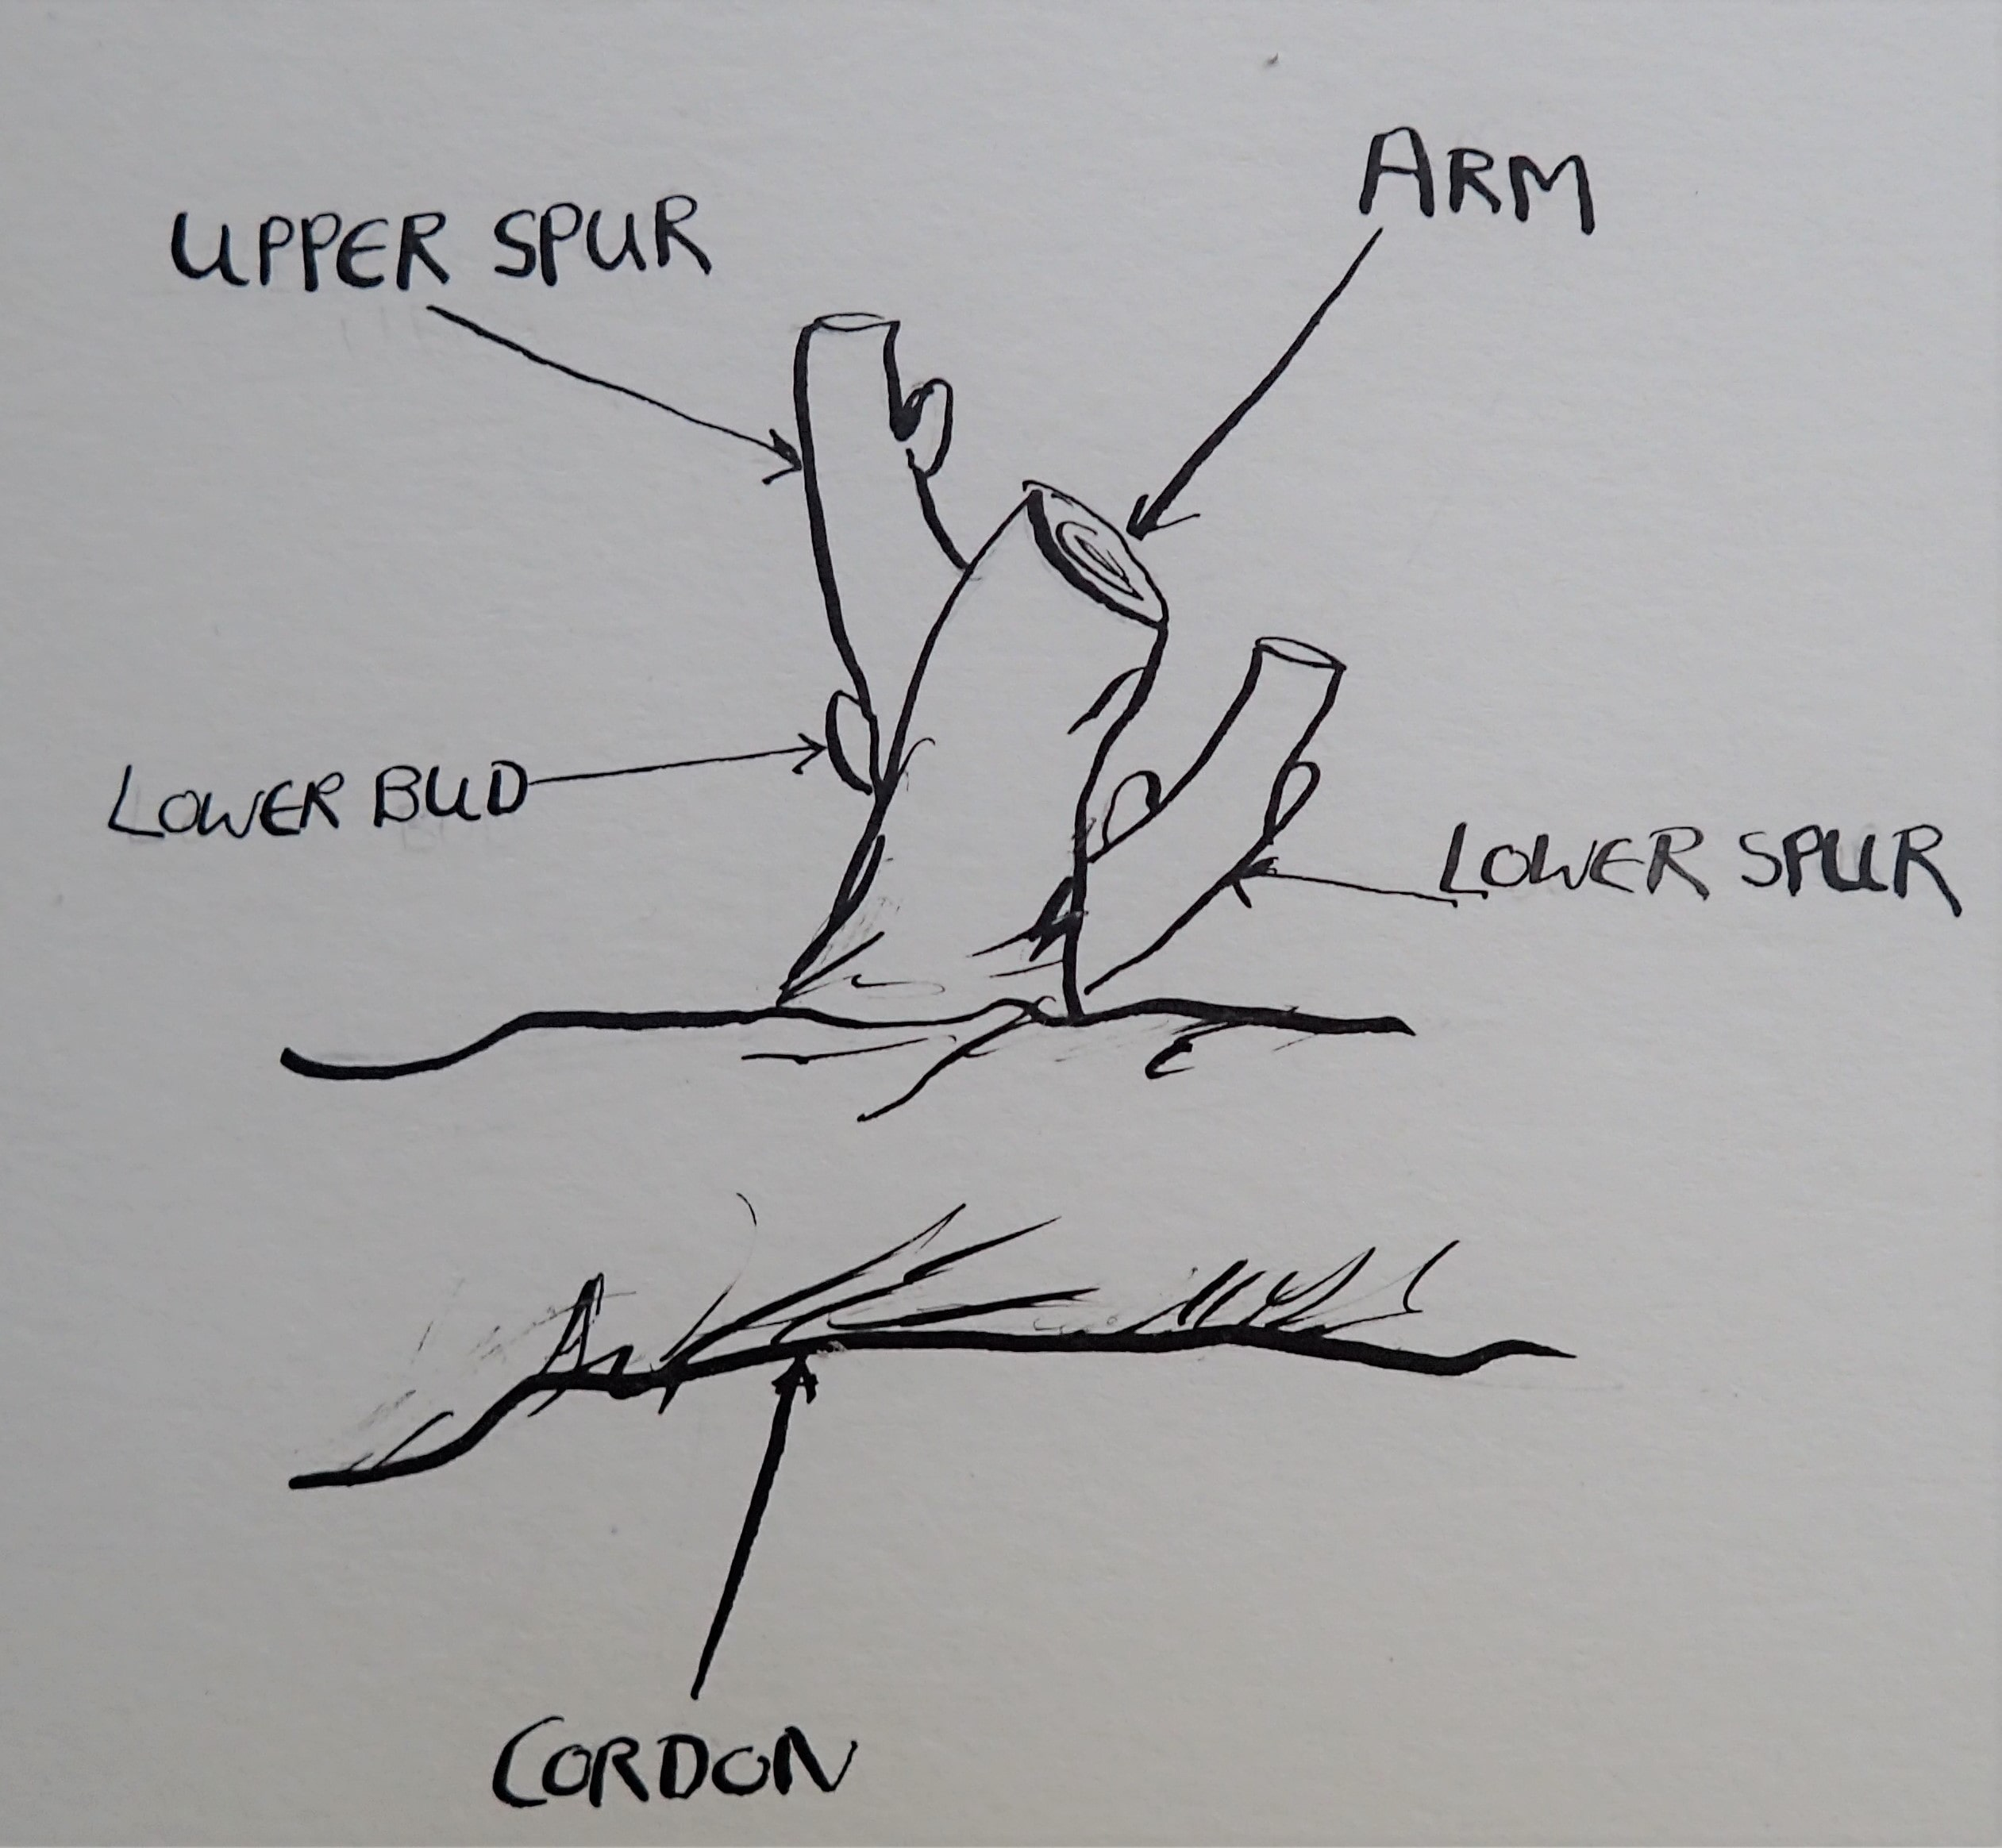
\includegraphics[width=\linewidth]{TwoSpurs.jpg}
  \caption{A diagram of an arm of a cordon that had two spurs on it. In this case we chose to focus on the lower bud of the higher of the two spurs for monitoring. }
  \label{fig:TwoSpurs}
\end{figure}

\section{Finding the buds}
We flagged three buds/shoots on each of the vines in our monitoring program. We randomly chose one of the canes or cordons on each plant, and flagged three arms or spurs on the chosen cordon (Figure \ref{fig:CordonPruned}) or three buds/shoots on the chosen cane (Figure \ref{fig:CanePruned}). We flagged a bud close to the trunk, a middle bud, and the bud at the end of the cordon/cane. We flagged as close to the bud as we could when we initially placed the flagging tape, and later flagged some of the shoots once they were big enough. For the cordon pruned vines, we monitor the lowest bud/shoot of the highest spur of the arm (Figure \ref{fig:TwoSpurs}). If any of the flags are missing, figure out which bud position is missing and flag a bud in this position. Note the change on the datasheet.

\section{Selecting clusters to monitor flowering/veraison} % follow Davis protocol
\begin{enumerate}
	\item Once the shoot we are monitoring becomes well-developed (12 leaves and developed inflorescence), move the flagging to a specific inflorescence (cluster). This is probably best done as you move to monitoring \% flowering. 
	\item We will sample one cluster per shoot. Select the dominant cluster (usually the most basal cluster of the monitored cane/shoot); if during the season your cluster dies or is removed for some reason, select a nearby dominant cluster and make a note. 

\end{enumerate}

\section{Observing Phenology}
We are using the Eichorn-Lorenz system for monitoring phenology until flowering described in this PDF: \\

\begin{figure}%this will always show at this point 
  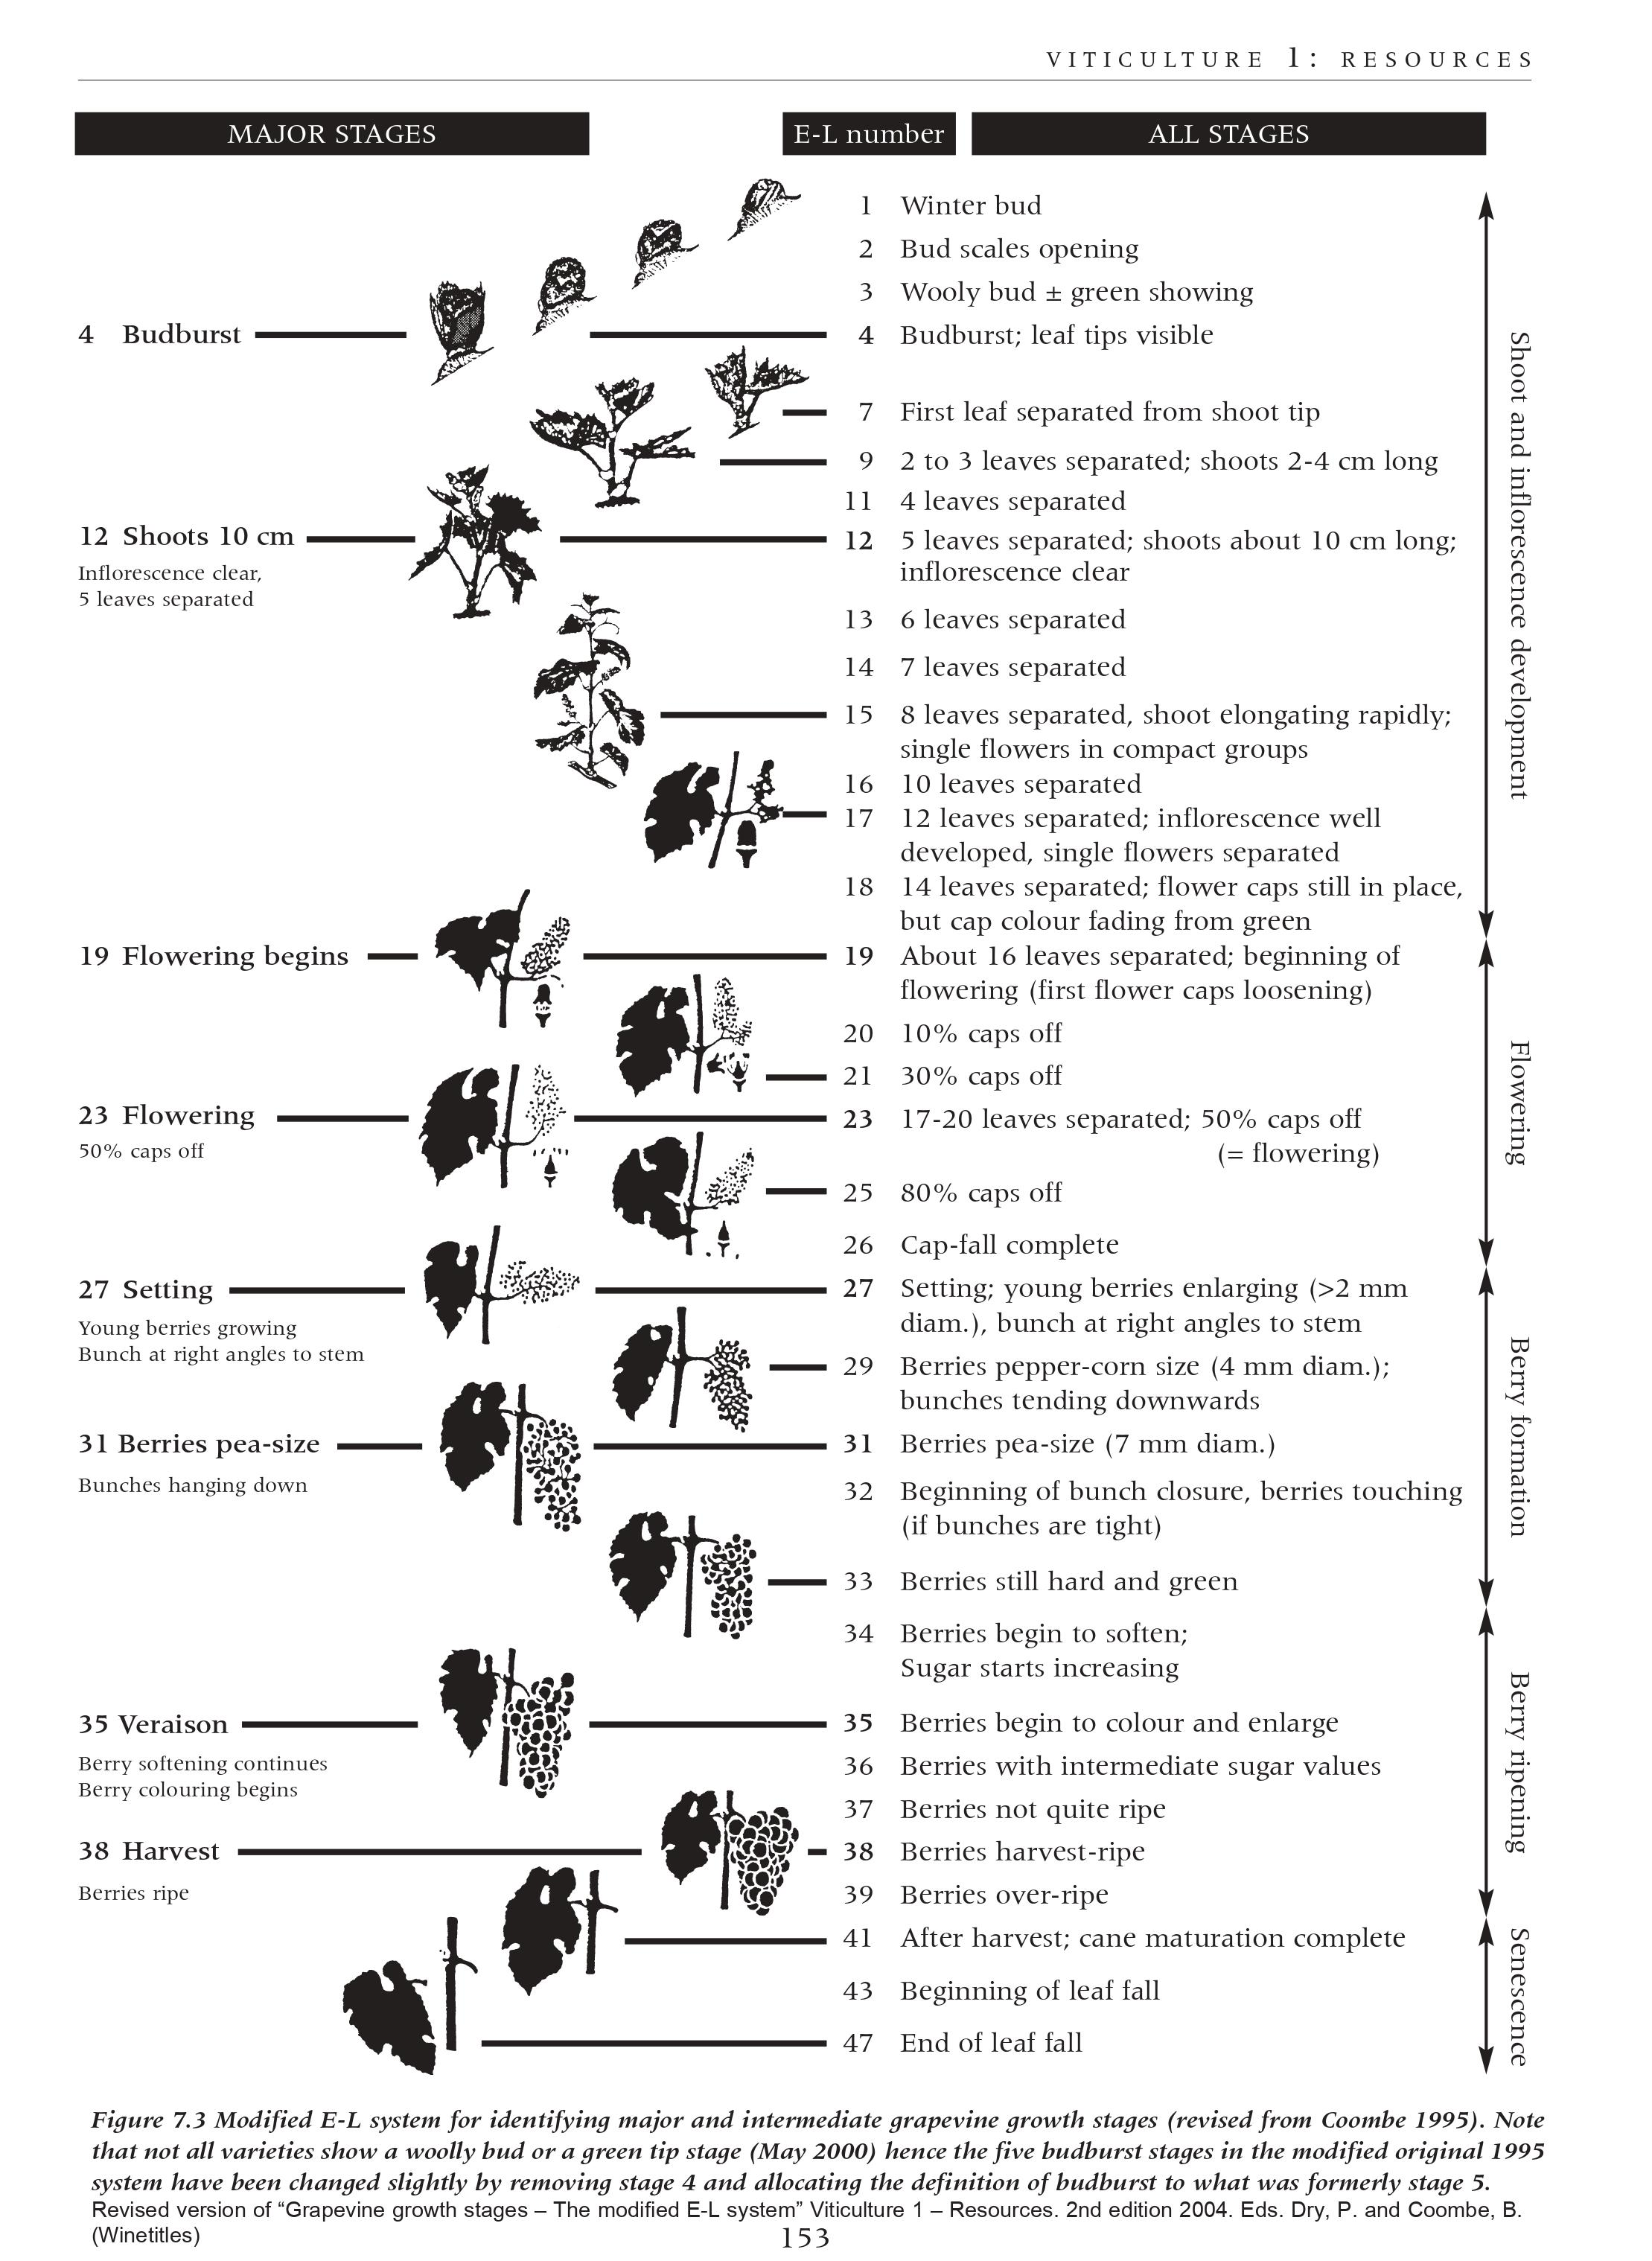
\includegraphics[width=\linewidth]{ELScale.jpg}
  \caption{ Modified Eichorn-Lorenz (EL) scale that our lab uses for monitoring phenology until flowering }
  \label{fig:ELScale}
\end{figure}

Our goal is to have standardized observations of phenological stages for analysis. There are four main widely observed stages for grapevine: (1) budburst, (2) flowering or bloom, (3) veraison, and (4) ripening and harvest. For the first stage, budburst, we will use the stage numbers from the Modified Eichorn-Lorenz system (a stage number between 1-17, with 4 meaning budburst; see Figure \ref{fig:ELScale} below).For stages 2 and 3, we will estimate the percent occurrence of the stage (proportion of berries on a selected cluster have gone through the stage of bloom or color change, respectively). We will measure ripening quantitatively, using a refractometer to measure Brix (sugar) accumulation. 

For each vine:
\begin{enumerate}
	\item Stand facing the vine. Double-check Plant ID (labeled with a sharpie on one of the flags), block, and row number before recording in correct place on data sheet that we will provide. We don't keep information on the varieties within each block on the field data recording sheets.
	\item Bud numbers are not written on the flags but are numbered 1 to 3 with Bud 1 being the most southern or eastern bud. (Not the easiest system but we're stuck with it for this summer)
	\item For pre-bloom, record the appropriate E-L stage of the shoot that was flagged, or the shoot closest to the flagging that matches our selection criteria laid out in the section above. Record its EL stage (number from “1”: still dormant, to “17”: twelve leaves separated- see \ref{fig:ELScale}) until EL stage 9. Once EL stage is at 9 you can stop recording until flowering starts (note that you may need to record higher than stage 9 at times in order to record whatever stage you see after 8, even if it is 12 or such if you have not yet recorded stage 9, more on this below).
	\item  For bloom (EL 23) and veraison (EL 35), look at each cluster (\#1, \#2, \#3) and estimate the percent (from 0-100\%) of berries on the sample cluster that have achieved that stage. 
	\item Take photos of representative illustrations for different varieties of target \% at stage (e.g., clusters at 5\%, 25\%, 50\%, 75\%, 95\% bloom) for different varieties. aim for 3-5 photos of each percentage taken across a diversity of varieties and across a couple different sampling dates, and make sure vine number and date are visible in photo for identification. {\bf Label the filename with the percent.}
	\item For ripening, our current plan is to send one of our team to collect berries so we can analyze Brix. We will aim to collect samples starting around 12-15 Brix until commercial harvest. % 18 Brix is quite high ... lower would be better!

\end{enumerate}


\section{What to do with the data}
After each round of monitoring, scan the datasheet and send to Mira. If you have taken photos, label them with the percent and the data then send them as well.

\section{Contact details}
Mira Garner - mira.garner@gmail.com, Cell: 608-228-5215


\end{document}

This is a short protocol designed for Mike and his team to continue gathering data while we are away. 
https://docs.google.com/document/d/13JRKCdJJOEcVo9Vh5Hub2SRHbJnhbqi8qDhj7a_kgiA/edit#